\documentclass[11pt,preprint, authoryear]{elsarticle}

\usepackage{lmodern}
%%%% My spacing
\usepackage{setspace}
\setstretch{1.2}
\DeclareMathSizes{12}{14}{10}{10}

% Wrap around which gives all figures included the [H] command, or places it "here". This can be tedious to code in Rmarkdown.
\usepackage{float}
\let\origfigure\figure
\let\endorigfigure\endfigure
\renewenvironment{figure}[1][2] {
    \expandafter\origfigure\expandafter[H]
} {
    \endorigfigure
}

\let\origtable\table
\let\endorigtable\endtable
\renewenvironment{table}[1][2] {
    \expandafter\origtable\expandafter[H]
} {
    \endorigtable
}


\usepackage{ifxetex,ifluatex}
\usepackage{fixltx2e} % provides \textsubscript
\ifnum 0\ifxetex 1\fi\ifluatex 1\fi=0 % if pdftex
  \usepackage[T1]{fontenc}
  \usepackage[utf8]{inputenc}
\else % if luatex or xelatex
  \ifxetex
    \usepackage{mathspec}
    \usepackage{xltxtra,xunicode}
  \else
    \usepackage{fontspec}
  \fi
  \defaultfontfeatures{Mapping=tex-text,Scale=MatchLowercase}
  \newcommand{\euro}{€}
\fi

\usepackage{amssymb, amsmath, amsthm, amsfonts}

\def\bibsection{\section*{References}} %%% Make "References" appear before bibliography


\usepackage[round]{natbib}

\usepackage{longtable}
\usepackage[margin=2.3cm,bottom=2cm,top=2.5cm, includefoot]{geometry}
\usepackage{fancyhdr}
\usepackage[bottom, hang, flushmargin]{footmisc}
\usepackage{graphicx}
\numberwithin{equation}{section}
\numberwithin{figure}{section}
\numberwithin{table}{section}
\setlength{\parindent}{0cm}
\setlength{\parskip}{1.3ex plus 0.5ex minus 0.3ex}
\usepackage{textcomp}
\renewcommand{\headrulewidth}{0.2pt}
\renewcommand{\footrulewidth}{0.3pt}

\usepackage{array}
\newcolumntype{x}[1]{>{\centering\arraybackslash\hspace{0pt}}p{#1}}

%%%%  Remove the "preprint submitted to" part. Don't worry about this either, it just looks better without it:
\makeatletter
\def\ps@pprintTitle{%
  \let\@oddhead\@empty
  \let\@evenhead\@empty
  \let\@oddfoot\@empty
  \let\@evenfoot\@oddfoot
}
\makeatother

 \def\tightlist{} % This allows for subbullets!

\usepackage{hyperref}
\hypersetup{breaklinks=true,
            bookmarks=true,
            colorlinks=true,
            citecolor=blue,
            urlcolor=blue,
            linkcolor=blue,
            pdfborder={0 0 0}}


% The following packages allow huxtable to work:
\usepackage{siunitx}
\usepackage{multirow}
\usepackage{hhline}
\usepackage{calc}
\usepackage{tabularx}
\usepackage{booktabs}
\usepackage{caption}


\newenvironment{columns}[1][]{}{}

\newenvironment{column}[1]{\begin{minipage}{#1}\ignorespaces}{%
\end{minipage}
\ifhmode\unskip\fi
\aftergroup\useignorespacesandallpars}

\def\useignorespacesandallpars#1\ignorespaces\fi{%
#1\fi\ignorespacesandallpars}

\makeatletter
\def\ignorespacesandallpars{%
  \@ifnextchar\par
    {\expandafter\ignorespacesandallpars\@gobble}%
    {}%
}
\makeatother

\newlength{\cslhangindent}
\setlength{\cslhangindent}{1.5em}
\newenvironment{CSLReferences}%
  {\setlength{\parindent}{0pt}%
  \everypar{\setlength{\hangindent}{\cslhangindent}}\ignorespaces}%
  {\par}


\urlstyle{same}  % don't use monospace font for urls
\setlength{\parindent}{0pt}
\setlength{\parskip}{6pt plus 2pt minus 1pt}
\setlength{\emergencystretch}{3em}  % prevent overfull lines
\setcounter{secnumdepth}{5}

%%% Use protect on footnotes to avoid problems with footnotes in titles
\let\rmarkdownfootnote\footnote%
\def\footnote{\protect\rmarkdownfootnote}
\IfFileExists{upquote.sty}{\usepackage{upquote}}{}

%%% Include extra packages specified by user
\usepackage{booktabs}
\usepackage{longtable}
\usepackage{array}
\usepackage{multirow}
\usepackage{wrapfig}
\usepackage{float}
\usepackage{colortbl}
\usepackage{pdflscape}
\usepackage{tabu}
\usepackage{threeparttable}
\usepackage{threeparttablex}
\usepackage[normalem]{ulem}
\usepackage{makecell}
\usepackage{xcolor}
\usepackage{caption}
\usepackage{graphicx}
\usepackage{siunitx}
\usepackage{hhline}
\usepackage{calc}
\usepackage{tabularx}
\usepackage{adjustbox}
\usepackage{hyperref}

%%% Hard setting column skips for reports - this ensures greater consistency and control over the length settings in the document.
%% page layout
%% paragraphs
\setlength{\baselineskip}{12pt plus 0pt minus 0pt}
\setlength{\parskip}{12pt plus 0pt minus 0pt}
\setlength{\parindent}{0pt plus 0pt minus 0pt}
%% floats
\setlength{\floatsep}{12pt plus 0 pt minus 0pt}
\setlength{\textfloatsep}{20pt plus 0pt minus 0pt}
\setlength{\intextsep}{14pt plus 0pt minus 0pt}
\setlength{\dbltextfloatsep}{20pt plus 0pt minus 0pt}
\setlength{\dblfloatsep}{14pt plus 0pt minus 0pt}
%% maths
\setlength{\abovedisplayskip}{12pt plus 0pt minus 0pt}
\setlength{\belowdisplayskip}{12pt plus 0pt minus 0pt}
%% lists
\setlength{\topsep}{10pt plus 0pt minus 0pt}
\setlength{\partopsep}{3pt plus 0pt minus 0pt}
\setlength{\itemsep}{5pt plus 0pt minus 0pt}
\setlength{\labelsep}{8mm plus 0mm minus 0mm}
\setlength{\parsep}{\the\parskip}
\setlength{\listparindent}{\the\parindent}
%% verbatim
\setlength{\fboxsep}{5pt plus 0pt minus 0pt}



\begin{document}



%titlepage
\thispagestyle{empty}
\begin{center}
\begin{minipage}{0.75\linewidth}
    \centering
%Entry1
    {\uppercase{\huge LATE to the Party: Investigating Instrument
Variables for Education\par}}
    \vspace{2cm}
%Author's name
    {\LARGE \textbf{Cassandra Pengelly}\par}
    \vspace{1cm}
%University logo
\begin{center}
    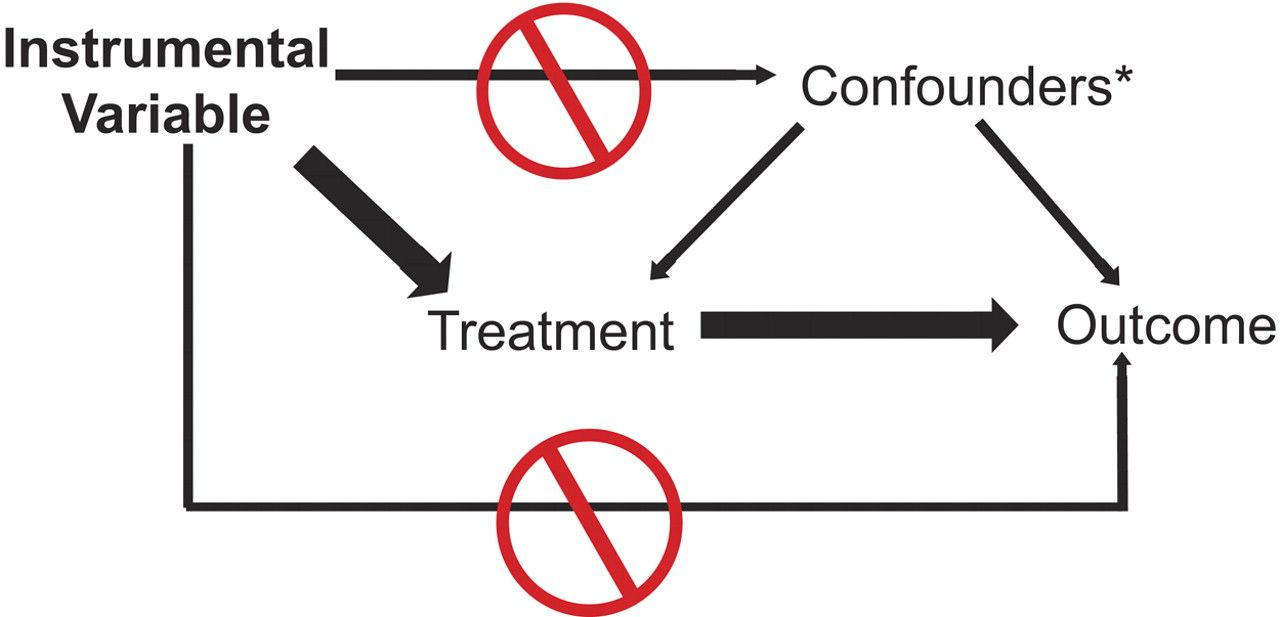
\includegraphics[width=1\linewidth]{Tex/logo.jpeg}
\end{center}
\vspace{1cm}
%Supervisor's Details
\begin{center}
    {\Large 20346212\par}
    \vspace{1cm}
%Degree
    {\large \textbf{Econometrics 871: Cross Section Project}\par}
    \vspace{1cm}
%Institution
    {\large Stellenbosch University\par}
    \vspace{1cm}
%Date
    {\large July 2021}
%More
    {\normalsize }
%More
    {\normalsize }
\end{center}
\end{minipage}
\end{center}
\clearpage


\begin{frontmatter}  %

\title{}

% Set to FALSE if wanting to remove title (for submission)


\vspace{1cm}





\vspace{0.5cm}

\end{frontmatter}


\renewcommand{\contentsname}{Table of Contents}
{\tableofcontents}

%________________________
% Header and Footers
%%%%%%%%%%%%%%%%%%%%%%%%%%%%%%%%%
\pagestyle{fancy}
\chead{}
\rhead{}
\lfoot{}
\rfoot{\footnotesize Page \thepage}
\lhead{}
%\rfoot{\footnotesize Page \thepage } % "e.g. Page 2"
\cfoot{}

%\setlength\headheight{30pt}
%%%%%%%%%%%%%%%%%%%%%%%%%%%%%%%%%
%________________________

\headsep 35pt % So that header does not go over title




\newpage

\hypertarget{introduction}{%
\section{\texorpdfstring{Introduction
\label{Introduction}}{Introduction }}\label{introduction}}

The return to education is a cornerstone topic in labour economics and
is of particular interest to policymakers. This is no different in South
Africa, especially given the significant income inequality, which is
often claimed to be strongly linked to differences in education.
However, wages cannot simply be regressed on education because there is
likely endogeneity present. This arises from the problem of there being
an omitted variable, where education and wages are both correlated with
a variable in the error term. One variable of this nature that has been
extensively studied is innate ability
(\protect\hyperlink{ref-hertz}{Hertz}
(\protect\hyperlink{ref-hertz}{2003})). Returns to schooling could be
biased upwards if ability is positively correlated with both income and
education. However, as \protect\hyperlink{ref-disc}{Lang}
(\protect\hyperlink{ref-disc}{1993}) assesses, the overall findings of
research on the impact of ability bias are inconclusive. In fact,
\protect\hyperlink{ref-disc}{Lang} (\protect\hyperlink{ref-disc}{1993:
1}) notes that several papers find that returns to education are
\emph{downwardly} biased.

This paper will investigate whether OLS estimates are biased in the
South African case by estimating the return to education using four
different instrumental variable estimators: the first two exploit
parents' education, and the other two use parents' occupations. These
instruments estimate a `local average treatment effect', which - this
paper will argue - is more appropriate than OLS estimators for analysing
the returns to education for South Africa, if certain assumptions are
met. These instruments are tested for strength and validity and then
implemented on the NIDS Wave 5 data set. This essay\footnote{This essay
  was written in R using the Texevier package by
  \protect\hyperlink{ref-Texevier}{Katzke}
  (\protect\hyperlink{ref-Texevier}{2017})} is structured as follows:
section \ref{data} details the data set used and discusses the
descriptive statistics. Section \ref{meth} outlines the methodology and
investigates whether the LATE assumptions for the instrumental variables
hold. Following this, section \ref{results} discusses the regression
results and evaluates the robustness of the estimators used to obtain a
causal effect. The final section, \ref{conclusion},
concludes\footnote{The code and write up for this project can be found
  on Github \url{https://github.com/cass-code/Cross-Section.git}}.

\hypertarget{data}{%
\section{\texorpdfstring{Data \label{data}}{Data }}\label{data}}

The data used for this paper is sourced from the National Income
Dynamics Survey (NIDS) (\protect\hyperlink{ref-nids}{\emph{National
income dynamics study 2017, wave 5 dataset}}
(\protect\hyperlink{ref-nids}{2018})), which was the first national
household panel study in South Africa. NIDS is an initiative of the
Department of Planning, Monitoring and Evaluation, and the Southern
Africa Labour and Development Research Unit (SALDRU) is tasked with its
implementation (\protect\hyperlink{ref-nids5}{Brophy, Branson, Daniels,
Leibbrandt, Mlatsheni \& Woolard}
(\protect\hyperlink{ref-nids5}{2018})). NIDS was started in 2008, with
over 28,000 people interviewed. These same people are then interviewed
every two years. The latest survey is Wave 5 (2017), which is the data
set used for the regression analysis, where the individual is the unit
of observation. Wave 5 consists of 37,368 individuals, where the high
rate of attrition among high-income, Indian/Asian, and White respondents
has led to the sample being increased by 2,775 to maintain sample
representativeness (\protect\hyperlink{ref-nids5}{Brophy, Branson,
Daniels, Leibbrandt, Mlatsheni \& Woolard}
(\protect\hyperlink{ref-nids5}{2018})).

\protect\hyperlink{ref-nids1}{Villiers, Leibbrandt \& Woolard}
(\protect\hyperlink{ref-nids1}{2009}) outlay the design of the survey.
To sample the households used in Wave 1, two-stage cluster sample design
with stratification was employed. Stage 1 involved selecting 400 Primary
Sampling Units, based on Statistics South Africa's Master Sample of
Primary Sampling Units (2003). Private households in all of South
Africa's 9 provinces are the target population for NIDS. The 53
disctrict councils make up the explicit strata in the Master sample.
Based on the allocation of the district councils in the Primary Sampling
Units in the Master Sample, the sample was proportionally allocated and
the Primary Sampling Units were randomly chosen within the strata
(\protect\hyperlink{ref-nids1}{Villiers, Leibbrandt \& Woolard}
(\protect\hyperlink{ref-nids1}{2009}) p.9). Fieldworkers are assigned to
the selected addresses and are instructed to interview all households
living at the dwelling unit.

The NIDS wave 5 data set contains 30,110 observations of 1,144
variables. As a part of the data cleaning process, I selected 14
variables: year of birth, gender, race, income, marital status, highest
level of schooling, highest level of tertiary education, union status,
father's schooling, father's tertiary education, father's occupation,
mother's schooling, mother's tertiary education, and mother's
occupation. The occupation variables have been re-coded with the
appropriate profession names from the
\protect\hyperlink{ref-isco}{\emph{International standard classification
of occupations}} (\protect\hyperlink{ref-isco}{2012}), and are therefore
categorical variables. I constructed the variables age and age-squared
from the year of birth, and I constructed an education variable, which
represents the number of years of education for an individual
(i.e.~summing the years of schooling and years of tertiary education). I
constructed a similar variable for mother and father's education.
Unfortunately, there are a significant number of missing observations
for the variables income, parents' education, marital status and union
status. Because of this, the sample size for the regressions is reduced
to 3,300 and under.

As a part of the initial data exploration, figure \ref{Figure1} gives a
quick snapshot of the relationship between income and education. As
shown by the black regression line, income and education are positively
correlated, which is what we expect. Section \ref{results} will argue
that this is a causal relationship. We can also glimpse how education
and income are distributed in the sample. To get a clearer view of the
race distribution, figure \ref{Figure2} shows a bar plot of the four
main race groups in South Africa: African, Asian/Indian, Coloured and
White. The graph shows the sample is roughly representative of the South
African population, with a slightly smaller sample of Asian/Indian and
White individuals (despite the top up sample). We also want to check
that income is normally distributed to combat heteroskedasticity in the
regression analysis. We find that the income distribution is skewed but
log of income is fairly normal, as figure \ref{Figure3} shows. This
indicates that log of income should be the dependent variable in the
regressions (rather the linear form of income), which is also supported
by the literature.

\begin{figure}[H]

{\centering \includegraphics{20346212CSproj_files/figure-latex/lineargraph-1} 

}

\caption{Income and Education Relationship \label{Figure1}}\label{fig:lineargraph}
\end{figure}

\begin{figure}[H]

{\centering \includegraphics{20346212CSproj_files/figure-latex/racegraph-1} 

}

\caption{Race Proportions of Sample \label{Figure2}}\label{fig:racegraph}
\end{figure}

\begin{figure}[H]

{\centering \includegraphics{20346212CSproj_files/figure-latex/incomergraph-1} 

}

\caption{Log Income Distribution  \label{Figure3}}\label{fig:incomergraph}
\end{figure}

\hypertarget{methodology}{%
\section{\texorpdfstring{Methodology
\label{meth}}{Methodology }}\label{methodology}}

Following the earnings function proposed by
\protect\hyperlink{ref-mince}{Mincer}
(\protect\hyperlink{ref-mince}{1974}), to model the relationship between
income and education in \ref{reg1}, the following general OLS
regression, \ref{eq1}, is used: \begin{align}
Log(income)=\beta_{0}+\beta_{1} X_{1}+\cdots+\beta_{k} X_{k}+u  \label{eq1}
\end{align} where \(X_{1}\) is education and \(\ldots, X_{k}\) includes
the other regressors: age, age-squared, race and gender,
\(\beta_{0}, \ldots, \beta_{k}\) are the regression coefficients, and
\(u\) is the error term. Race is a categorical variable with the
reference group as African, and gender is a dummy variable that takes a
value of 1 if an individual is male and 0 otherwise.

If education is an endogenous regressor - i.e.~correlated with the error
term - then the OLS coefficient for education (\(\beta_{1}\)) will be
biased (\protect\hyperlink{ref-R}{Colonescu}
(\protect\hyperlink{ref-R}{2016})). If we can find an instrumental
variable for education, then we can remove this endogeneity and get an
unbiased coefficient for education
(\protect\hyperlink{ref-metrics}{Stock \& Watson}
(\protect\hyperlink{ref-metrics}{2015}) \&
\protect\hyperlink{ref-metrics1}{Venables \& Smith}
(\protect\hyperlink{ref-metrics1}{2010})). 4 different variables are
used as an instrument for an individual's education: father's education,
mother's education, father's occupation and mother's occupation. In
order to use these variables as instruments, we have to check their
validity (\protect\hyperlink{ref-ang}{Imbens \& Angrist}
(\protect\hyperlink{ref-ang}{1994})). Economic theory and the literature
suggests that returns to schooling are heterogeneous
(\protect\hyperlink{ref-return}{Koop \& Tobias}
(\protect\hyperlink{ref-return}{2004: 827--828})), which implies that
for the instruments to be valid they have to comply with the Local
Average Treatment Effects (LATE) identifying assumptions. The four LATE
assumptions are: relevance, monotonicity, random assignment and
exclusion restriction. The section below, \ref{spec}, interprets the
diagnostic tests for the instrument variables and evaluates whether the
LATE assumptions hold.

\hypertarget{specification-tests-and-late-assumptions}{%
\subsection{\texorpdfstring{Specification Tests and LATE
Assumptions\label{spec}}{Specification Tests and LATE Assumptions}}\label{specification-tests-and-late-assumptions}}

The relevance assumption is directly testable on the data, for which we
can use the `Weak Instrument' test. The results of the specification
tests in the appendix, \ref{appendixA}, show that all four instruments
are not weak instruments. The null hypothesis for the `Weak Instrument'
test is that the instrument is weak. The p-values for each of the
individual tests are zero, which rejects the null hypothesis. This
supports the relevance assumption and these instruments affect treatment
for at least some individuals. This makes intuitive sense as well: if an
individual was on the fence about studying further, and his/her parents
studied further, the parents are likely to convince that individual to
follow in their footsteps/take the ``safe'' option of studying further.

The Wu-Hausman test evaluates whether the OLS and instrumental variable
regressions give significantly different estimates. The null hypothesis
is that the estimated coefficients of OLS and IV regression are not
statistically different from one another. For all four instruments, the
null hypothesis is rejected, which means the OLS and IV estimates are
sufficiently different from one another. The Sargan test is applicable
when the number of instruments exceeds the number of endogenous
variables. Rejecting the null of the Sargan test implies that the
instruments are invalid. For father's occupation and mother's
occupation, the Sargan test fails to reject the null, thus all the
instrumental variables are valid.

Regarding the assumption of monotonicity: it seems unlikely that someone
who would have pursued education further would decide not to because
either of his/her parents pursued education further. Thus, it is
reasonable to conclude that the monotonicity assumption holds for
father's and mother's education (i.e.~there are no defiers). Similarly,
it seems unreasonable that someone who would have pursued education
further would decide not to due to his/her parents' occupation.
Although, one could argue that: if an individual would have liked to
study further, but doesn't want the pressure of living up to his/her
parents' academic achievements and so opts out, the monotonicity
assumption is invalid. However, this is unlikely to occur for the
majority of the sample and can be ignored.

The random assignment assumption is difficult to argue for, since the
distribution of potential outcomes and potential take-up values should
look same for those whose parents studied further and for those whose
didn't, when in reality the distribution doesn't look the same. We would
expect individuals whose parents have lower levels of education to have
different potential earnings distributions or potential take-up
probabilities than individuals whose parents have higher levels of
education. Similarly for individual's whose parents have different
occupations. In South Africa, networks play a large role in employment
opportunities and therefore play a role in earning potentials. The
earnings' potential of an individual changes depending on their
connections and their parents' connections, which is correlated to
parental occupation; this is a violation of the exclusion restriction.

The exclusion restriction assumption is broken if an individual's
parents' education affects his/her potential earnings through another
variable other than education. This is possible, for example, through
socioeconomic standing. If an individual's parents' education/occupation
is correlated with their being wealthy and well-connected, and having
wealthy and well-connected parents increases earning potential (they
could provide financial and social capital for business ventures) then
the exclusion restriction assumption no longer holds. However, according
to \protect\hyperlink{ref-block}{Hoogerheide, Block \& Thurik}
(\protect\hyperlink{ref-block}{2012}), violations of the strict validity
assumption does not necessarily lead to results which differ
significantly from those of the strict validity case.
\protect\hyperlink{ref-block}{Hoogerheide, Block \& Thurik}
(\protect\hyperlink{ref-block}{2012}) make the case that family
background variables can be used as instruments for regressions
involving income. The next section \ref{results} discusses the results
of the ordinary least squares regression (OLS) compared to the
instrumental variable (IV )regressions.

\hypertarget{results}{%
\section{\texorpdfstring{Results
\label{results}}{Results }}\label{results}}

Table \ref{FE} in the appendix (\ref{appendix}) presents the regression
results, and the figure below it plots the regression coefficients with
their 95\% confidence intervals. The OLS regression regresses log income
on education, controlling for age, race, and gender. The coefficients of
the control variables have the expected signs and most are statistically
significant at 1\%. The coefficient for education is 0.194, which
implies that a 1 unit (a year) increase in education is associated with
a 21,4\% increase in income, ceteris paribus. However, in order to show
there exists a causal relationship between education and income, and
that there exists bias in the OLS estimate, two-stage least squares
(2SLS) was applied using the 4 different instrumental variables.

The first 2SLS regression employs father's education as an instrument
for education (2SLS FE in \ref{reg1}). The coefficient for this
regression is 0.309, which is significantly higher than the OLS
estimate. This implies that the OLS estimate is bias downwards. The
second IV regression uses mother's education as an instrument for
education (2SLS ME in \ref{reg1}). The coefficient for education here is
0.280; again this is a lot higher than the OLS estimate. The third and
fourth 2SLS regressions that exploit father's and mother's occupation as
instrument variables for education (2SLS FO, 2SLS MO in \ref{reg1}) show
similar results. They estimate the coefficient for education to be 0.327
and 0.387 respectively. However, the sample size diminishes when using
occupation as a variable, which makes them less statistically
trustworthy than the other estimates. This is illustrated clearly by the
large confidence bands for `FO' and `MO' in the figure in the appendix
\ref{reg1}. Overall, the IV regression results show that the OLS
estimate is substantially downwards biased. These findings are similar
to those of \protect\hyperlink{ref-agree}{Biyase \& Zwane}
(\protect\hyperlink{ref-agree}{2015}), who also show that returns to
education are underreported by OLS regressions.

However, it is important to recognize that the 2SLS estimators recover
local average treatment effects (LATE) whereas OLS estimators recover
average treatment effects. In the IV regressions, the effect of further
education is only captured for those individuals who are more likely to
further their education because their parents pursued education further.
This empirical stance does not provide information about the effect of
studying further among people would have always studied further or never
studied further, regardless of their parents' education/occupations.

\hypertarget{conclusion}{%
\section{\texorpdfstring{Conclusion
\label{conclusion}}{Conclusion }}\label{conclusion}}

This essay set out to show that there is a causal link between education
and income using four different instrumental variables. The OLS
regression finds that education has a positive coefficient, as expected,
but the four 2SLS regressions indicate that OLS may be underestimating
the returns to education. The fact that all four 2SLS regressions show
higher education estimates suggests the results are robust, and the
instrumental variables shift the estimate enough to indicate that OLS
would be inconsistent. Although some of the LATE assumptions may be
violated by selecting parents' education and occupations as instrumental
variables, they may still be viable tools to introduce exogeneity into
the model (\protect\hyperlink{ref-block}{Hoogerheide, Block \& Thurik}
(\protect\hyperlink{ref-block}{2012})). Further robustness checks could
be conducted by including more controls in the regressions (such as
marital status and union status\footnote{I ran these regressions and
  found similar results; however the sample sizes were very small}),
using fixed effects to control for time invariant unobservables or using
education lagged as an instrument variable.

\newpage

\hypertarget{references}{%
\section*{References}\label{references}}
\addcontentsline{toc}{section}{References}

\hypertarget{refs}{}
\begin{CSLReferences}{1}{0}
\leavevmode\hypertarget{ref-agree}{}%
Biyase, M. \& Zwane, T. 2015. Does education pay in south africa?
Estimating returns to education using two stage least squares approach.
\emph{International Business \& Economics Research Journal (IBER)}.
14(6):807--814.

\leavevmode\hypertarget{ref-nids5}{}%
Brophy, T., Branson, N., Daniels, R.C., Leibbrandt, M., Mlatsheni, C. \&
Woolard, I. 2018. \emph{National income dynamics study panel user
manual}. (Release 2018. Version 1). Cape Town: Southern Africa Labour;
Development Research Unit; Southern Africa Labour; Development Research
Unit.

\leavevmode\hypertarget{ref-R}{}%
Colonescu, C. 2016. Principles of econometrics with r. 11. {[}Online{]},
Available: \url{https://bookdown.org/ccolonescu/RPoE4/}.

\leavevmode\hypertarget{ref-hertz}{}%
Hertz, T. 2003. Upward bias in the estimated returns to education:
Evidence from south africa. \emph{American Economic Review}.
93(4):1354--1368.

\leavevmode\hypertarget{ref-block}{}%
Hoogerheide, L., Block, J. \& Thurik, R. 2012. Family background
variables as instruments for education in income regressions: A bayesian
analysis. \emph{Economics of Education Review}. 31(5):515--523.

\leavevmode\hypertarget{ref-ang}{}%
Imbens, G.W. \& Angrist, J.D. 1994. Identification and estimation of
local average treatment effects. \emph{Econometrica}. 62(2):467--475.
{[}Online{]}, Available: \url{http://www.jstor.org/stable/2951620}.

\leavevmode\hypertarget{ref-isco}{}%
\emph{International standard classification of occupations: Structure,
group definitions and correspondence tables}. 2012. (ISCO - 08).
International Labour Office, Geneva; International Labour Organization.

\leavevmode\hypertarget{ref-Texevier}{}%
Katzke, N.F. 2017. \emph{{Texevier}: {P}ackage to create elsevier
templates for rmarkdown}. Stellenbosch, South Africa: Bureau for
Economic Research.

\leavevmode\hypertarget{ref-return}{}%
Koop, G. \& Tobias, J.L. 2004. Learning about heterogeneity in returns
to schooling. \emph{Journal of Applied Econometrics}. 19(7):827--849.
{[}Online{]}, Available: \url{http://www.jstor.org/stable/25146329}.

\leavevmode\hypertarget{ref-disc}{}%
Lang, K. 1993. \emph{Ability bias, discount rate bias and the return to
education}. (MPRA Paper). University Library of Munich, Germany.
{[}Online{]}, Available:
\url{https://EconPapers.repec.org/RePEc:pra:mprapa:24651}.

\leavevmode\hypertarget{ref-mince}{}%
Mincer, J. 1974. \emph{Schooling, experience and earnings}. National
Bureau of Economics, New York: Columbia University Press.

\leavevmode\hypertarget{ref-nids}{}%
\emph{National income dynamics study 2017, wave 5 dataset}. 2018. Cape
Town, South Africa: Department of Planning, Monitoring,; Evaluation
{[}funding agency{]} \& DataFirst {[}distributor{]}. {[}Online{]},
Available: \url{https://doi.org/10.25828/fw3h-v708}.

\leavevmode\hypertarget{ref-metrics}{}%
Stock, J. H. \& Watson, M.W. 2015. \emph{Introduction to econometrics,
third update, global edition}. Pearson Education Limited.

\leavevmode\hypertarget{ref-metrics1}{}%
Venables, W.N. \& Smith, D.M. 2010. \emph{{R-Intro}: {A}n introduction
to r}. {[}Online{]}, Available:
\url{https://cran.r-project.org/doc/manuals/r-release/R-intro.pdf}.

\leavevmode\hypertarget{ref-nids1}{}%
Villiers, L. de, Leibbrandt, M. \& Woolard, I. 2009. \emph{Methodology:
Report on NIDS wave 1}. (Technical Paper no. 1). Cape Town: Southern
Africa Labour; Development Research Unit; Southern Africa Labour;
Development Research Unit.

\end{CSLReferences}

\newpage

\hypertarget{appendix-a-specification-tests}{%
\section*{\texorpdfstring{Appendix A: Specification Tests
\label{appendixA}}{Appendix A: Specification Tests }}\label{appendix-a-specification-tests}}
\addcontentsline{toc}{section}{Appendix A: Specification Tests
\label{appendixA}}

\begin{table}

\caption{\label{tab:Specification}Specification Tests for Father's Education \label{FE}}
\centering
\begin{tabular}[t]{l|r|r|r|r}
\hline
  & df1 & df2 & statistic & p-value\\
\hline
Weak instruments & 1 & 3368 & 406.13620 & 0\\
\hline
Wu-Hausman & 1 & 3367 & 70.06385 & 0\\
\hline
Sargan & 0 & NA & NA & NA\\
\hline
\end{tabular}
\end{table}

\begin{table}

\caption{\label{tab:Specification}Specification Tests for Mother's Education \label{ME}}
\centering
\begin{tabular}[t]{l|r|r|r|r}
\hline
  & df1 & df2 & statistic & p-value\\
\hline
Weak instruments & 1 & 3605 & 400.15525 & 0\\
\hline
Wu-Hausman & 1 & 3604 & 46.19299 & 0\\
\hline
Sargan & 0 & NA & NA & NA\\
\hline
\end{tabular}
\end{table}

\begin{table}

\caption{\label{tab:Specification}Specification Tests for Father's Occupation \label{FO}}
\centering
\begin{tabular}[t]{l|r|r|r|r}
\hline
  & df1 & df2 & statistic & p-value\\
\hline
Weak instruments & 9 & 2162 & 19.86956 & 0.0000000\\
\hline
Wu-Hausman & 1 & 2169 & 32.61388 & 0.0000000\\
\hline
Sargan & 8 & NA & 12.65711 & 0.1242046\\
\hline
\end{tabular}
\end{table}

\begin{table}

\caption{\label{tab:Specification}Specification Tests for Mother's Occupation \label{MO}}
\centering
\begin{tabular}[t]{l|r|r|r|r}
\hline
  & df1 & df2 & statistic & p-value\\
\hline
Weak instruments & 9 & 1731 & 38.61704 & 0.000000\\
\hline
Wu-Hausman & 1 & 1738 & 64.04297 & 0.000000\\
\hline
Sargan & 8 & NA & 4.50194 & 0.809239\\
\hline
\end{tabular}
\end{table}

\hypertarget{appendix-b-regression-tables}{%
\section*{\texorpdfstring{Appendix B: Regression Tables
\label{appendix}}{Appendix B: Regression Tables }}\label{appendix-b-regression-tables}}
\addcontentsline{toc}{section}{Appendix B: Regression Tables
\label{appendix}}

 
  \providecommand{\huxb}[2]{\arrayrulecolor[RGB]{#1}\global\arrayrulewidth=#2pt}
  \providecommand{\huxvb}[2]{\color[RGB]{#1}\vrule width #2pt}
  \providecommand{\huxtpad}[1]{\rule{0pt}{#1}}
  \providecommand{\huxbpad}[1]{\rule[-#1]{0pt}{#1}}

\begin{table}[ht]
\begin{centerbox}
\begin{threeparttable}
\captionsetup{justification=centering,singlelinecheck=off}
\caption{Regressions: OLS and 2SLS with Various Instruments}
 \label{reg1}
\setlength{\tabcolsep}{0pt}
\begin{tabular}{l l l l l l}


\hhline{>{\huxb{0, 0, 0}{0.8}}->{\huxb{0, 0, 0}{0.8}}->{\huxb{0, 0, 0}{0.8}}->{\huxb{0, 0, 0}{0.8}}->{\huxb{0, 0, 0}{0.8}}->{\huxb{0, 0, 0}{0.8}}-}
\arrayrulecolor{black}

\multicolumn{1}{!{\huxvb{0, 0, 0}{0}}c!{\huxvb{0, 0, 0}{0}}}{\huxtpad{6pt + 1em}\centering \hspace{6pt} {\fontsize{12pt}{14.4pt}\selectfont } \hspace{6pt}\huxbpad{6pt}} &
\multicolumn{1}{c!{\huxvb{0, 0, 0}{0}}}{\huxtpad{6pt + 1em}\centering \hspace{6pt} {\fontsize{12pt}{14.4pt}\selectfont OLS} \hspace{6pt}\huxbpad{6pt}} &
\multicolumn{1}{c!{\huxvb{0, 0, 0}{0}}}{\huxtpad{6pt + 1em}\centering \hspace{6pt} {\fontsize{12pt}{14.4pt}\selectfont 2SLS FE} \hspace{6pt}\huxbpad{6pt}} &
\multicolumn{1}{c!{\huxvb{0, 0, 0}{0}}}{\huxtpad{6pt + 1em}\centering \hspace{6pt} {\fontsize{12pt}{14.4pt}\selectfont 2SLS ME} \hspace{6pt}\huxbpad{6pt}} &
\multicolumn{1}{c!{\huxvb{0, 0, 0}{0}}}{\huxtpad{6pt + 1em}\centering \hspace{6pt} {\fontsize{12pt}{14.4pt}\selectfont 2SLS FO} \hspace{6pt}\huxbpad{6pt}} &
\multicolumn{1}{c!{\huxvb{0, 0, 0}{0}}}{\huxtpad{6pt + 1em}\centering \hspace{6pt} {\fontsize{12pt}{14.4pt}\selectfont 2SLS MO} \hspace{6pt}\huxbpad{6pt}} \tabularnewline[-0.5pt]


\hhline{>{\huxb{255, 255, 255}{0.4}}->{\huxb{0, 0, 0}{0.4}}->{\huxb{0, 0, 0}{0.4}}->{\huxb{0, 0, 0}{0.4}}->{\huxb{0, 0, 0}{0.4}}->{\huxb{0, 0, 0}{0.4}}-}
\arrayrulecolor{black}

\multicolumn{1}{!{\huxvb{0, 0, 0}{0}}l!{\huxvb{0, 0, 0}{0}}}{\huxtpad{6pt + 1em}\raggedright \hspace{6pt} {\fontsize{12pt}{14.4pt}\selectfont Age} \hspace{6pt}\huxbpad{6pt}} &
\multicolumn{1}{r!{\huxvb{0, 0, 0}{0}}}{\huxtpad{6pt + 1em}\raggedleft \hspace{6pt} {\fontsize{12pt}{14.4pt}\selectfont 0.047 ***} \hspace{6pt}\huxbpad{6pt}} &
\multicolumn{1}{r!{\huxvb{0, 0, 0}{0}}}{\huxtpad{6pt + 1em}\raggedleft \hspace{6pt} {\fontsize{12pt}{14.4pt}\selectfont 0.040 ***} \hspace{6pt}\huxbpad{6pt}} &
\multicolumn{1}{r!{\huxvb{0, 0, 0}{0}}}{\huxtpad{6pt + 1em}\raggedleft \hspace{6pt} {\fontsize{12pt}{14.4pt}\selectfont 0.049 ***} \hspace{6pt}\huxbpad{6pt}} &
\multicolumn{1}{r!{\huxvb{0, 0, 0}{0}}}{\huxtpad{6pt + 1em}\raggedleft \hspace{6pt} {\fontsize{12pt}{14.4pt}\selectfont 0.056 ***} \hspace{6pt}\huxbpad{6pt}} &
\multicolumn{1}{r!{\huxvb{0, 0, 0}{0}}}{\huxtpad{6pt + 1em}\raggedleft \hspace{6pt} {\fontsize{12pt}{14.4pt}\selectfont 0.072 ***} \hspace{6pt}\huxbpad{6pt}} \tabularnewline[-0.5pt]


\hhline{}
\arrayrulecolor{black}

\multicolumn{1}{!{\huxvb{0, 0, 0}{0}}l!{\huxvb{0, 0, 0}{0}}}{\huxtpad{6pt + 1em}\raggedright \hspace{6pt} {\fontsize{12pt}{14.4pt}\selectfont } \hspace{6pt}\huxbpad{6pt}} &
\multicolumn{1}{r!{\huxvb{0, 0, 0}{0}}}{\huxtpad{6pt + 1em}\raggedleft \hspace{6pt} {\fontsize{12pt}{14.4pt}\selectfont (0.009)~~~} \hspace{6pt}\huxbpad{6pt}} &
\multicolumn{1}{r!{\huxvb{0, 0, 0}{0}}}{\huxtpad{6pt + 1em}\raggedleft \hspace{6pt} {\fontsize{12pt}{14.4pt}\selectfont (0.009)~~~} \hspace{6pt}\huxbpad{6pt}} &
\multicolumn{1}{r!{\huxvb{0, 0, 0}{0}}}{\huxtpad{6pt + 1em}\raggedleft \hspace{6pt} {\fontsize{12pt}{14.4pt}\selectfont (0.009)~~~} \hspace{6pt}\huxbpad{6pt}} &
\multicolumn{1}{r!{\huxvb{0, 0, 0}{0}}}{\huxtpad{6pt + 1em}\raggedleft \hspace{6pt} {\fontsize{12pt}{14.4pt}\selectfont (0.012)~~~} \hspace{6pt}\huxbpad{6pt}} &
\multicolumn{1}{r!{\huxvb{0, 0, 0}{0}}}{\huxtpad{6pt + 1em}\raggedleft \hspace{6pt} {\fontsize{12pt}{14.4pt}\selectfont (0.015)~~~} \hspace{6pt}\huxbpad{6pt}} \tabularnewline[-0.5pt]


\hhline{}
\arrayrulecolor{black}

\multicolumn{1}{!{\huxvb{0, 0, 0}{0}}l!{\huxvb{0, 0, 0}{0}}}{\huxtpad{6pt + 1em}\raggedright \hspace{6pt} {\fontsize{12pt}{14.4pt}\selectfont Age2} \hspace{6pt}\huxbpad{6pt}} &
\multicolumn{1}{r!{\huxvb{0, 0, 0}{0}}}{\huxtpad{6pt + 1em}\raggedleft \hspace{6pt} {\fontsize{12pt}{14.4pt}\selectfont -0.000 **~} \hspace{6pt}\huxbpad{6pt}} &
\multicolumn{1}{r!{\huxvb{0, 0, 0}{0}}}{\huxtpad{6pt + 1em}\raggedleft \hspace{6pt} {\fontsize{12pt}{14.4pt}\selectfont -0.000~~~~} \hspace{6pt}\huxbpad{6pt}} &
\multicolumn{1}{r!{\huxvb{0, 0, 0}{0}}}{\huxtpad{6pt + 1em}\raggedleft \hspace{6pt} {\fontsize{12pt}{14.4pt}\selectfont -0.000 *~~} \hspace{6pt}\huxbpad{6pt}} &
\multicolumn{1}{r!{\huxvb{0, 0, 0}{0}}}{\huxtpad{6pt + 1em}\raggedleft \hspace{6pt} {\fontsize{12pt}{14.4pt}\selectfont -0.000 *~~} \hspace{6pt}\huxbpad{6pt}} &
\multicolumn{1}{r!{\huxvb{0, 0, 0}{0}}}{\huxtpad{6pt + 1em}\raggedleft \hspace{6pt} {\fontsize{12pt}{14.4pt}\selectfont -0.000 **~} \hspace{6pt}\huxbpad{6pt}} \tabularnewline[-0.5pt]


\hhline{}
\arrayrulecolor{black}

\multicolumn{1}{!{\huxvb{0, 0, 0}{0}}l!{\huxvb{0, 0, 0}{0}}}{\huxtpad{6pt + 1em}\raggedright \hspace{6pt} {\fontsize{12pt}{14.4pt}\selectfont } \hspace{6pt}\huxbpad{6pt}} &
\multicolumn{1}{r!{\huxvb{0, 0, 0}{0}}}{\huxtpad{6pt + 1em}\raggedleft \hspace{6pt} {\fontsize{12pt}{14.4pt}\selectfont (0.000)~~~} \hspace{6pt}\huxbpad{6pt}} &
\multicolumn{1}{r!{\huxvb{0, 0, 0}{0}}}{\huxtpad{6pt + 1em}\raggedleft \hspace{6pt} {\fontsize{12pt}{14.4pt}\selectfont (0.000)~~~} \hspace{6pt}\huxbpad{6pt}} &
\multicolumn{1}{r!{\huxvb{0, 0, 0}{0}}}{\huxtpad{6pt + 1em}\raggedleft \hspace{6pt} {\fontsize{12pt}{14.4pt}\selectfont (0.000)~~~} \hspace{6pt}\huxbpad{6pt}} &
\multicolumn{1}{r!{\huxvb{0, 0, 0}{0}}}{\huxtpad{6pt + 1em}\raggedleft \hspace{6pt} {\fontsize{12pt}{14.4pt}\selectfont (0.000)~~~} \hspace{6pt}\huxbpad{6pt}} &
\multicolumn{1}{r!{\huxvb{0, 0, 0}{0}}}{\huxtpad{6pt + 1em}\raggedleft \hspace{6pt} {\fontsize{12pt}{14.4pt}\selectfont (0.000)~~~} \hspace{6pt}\huxbpad{6pt}} \tabularnewline[-0.5pt]


\hhline{}
\arrayrulecolor{black}

\multicolumn{1}{!{\huxvb{0, 0, 0}{0}}l!{\huxvb{0, 0, 0}{0}}}{\huxtpad{6pt + 1em}\raggedright \hspace{6pt} {\fontsize{12pt}{14.4pt}\selectfont Education} \hspace{6pt}\huxbpad{6pt}} &
\multicolumn{1}{r!{\huxvb{0, 0, 0}{0}}}{\huxtpad{6pt + 1em}\raggedleft \hspace{6pt} {\fontsize{12pt}{14.4pt}\selectfont 0.194 ***} \hspace{6pt}\huxbpad{6pt}} &
\multicolumn{1}{r!{\huxvb{0, 0, 0}{0}}}{\huxtpad{6pt + 1em}\raggedleft \hspace{6pt} {\fontsize{12pt}{14.4pt}\selectfont 0.309 ***} \hspace{6pt}\huxbpad{6pt}} &
\multicolumn{1}{r!{\huxvb{0, 0, 0}{0}}}{\huxtpad{6pt + 1em}\raggedleft \hspace{6pt} {\fontsize{12pt}{14.4pt}\selectfont 0.280 ***} \hspace{6pt}\huxbpad{6pt}} &
\multicolumn{1}{r!{\huxvb{0, 0, 0}{0}}}{\huxtpad{6pt + 1em}\raggedleft \hspace{6pt} {\fontsize{12pt}{14.4pt}\selectfont 0.327 ***} \hspace{6pt}\huxbpad{6pt}} &
\multicolumn{1}{r!{\huxvb{0, 0, 0}{0}}}{\huxtpad{6pt + 1em}\raggedleft \hspace{6pt} {\fontsize{12pt}{14.4pt}\selectfont 0.387 ***} \hspace{6pt}\huxbpad{6pt}} \tabularnewline[-0.5pt]


\hhline{}
\arrayrulecolor{black}

\multicolumn{1}{!{\huxvb{0, 0, 0}{0}}l!{\huxvb{0, 0, 0}{0}}}{\huxtpad{6pt + 1em}\raggedright \hspace{6pt} {\fontsize{12pt}{14.4pt}\selectfont } \hspace{6pt}\huxbpad{6pt}} &
\multicolumn{1}{r!{\huxvb{0, 0, 0}{0}}}{\huxtpad{6pt + 1em}\raggedleft \hspace{6pt} {\fontsize{12pt}{14.4pt}\selectfont (0.005)~~~} \hspace{6pt}\huxbpad{6pt}} &
\multicolumn{1}{r!{\huxvb{0, 0, 0}{0}}}{\huxtpad{6pt + 1em}\raggedleft \hspace{6pt} {\fontsize{12pt}{14.4pt}\selectfont (0.016)~~~} \hspace{6pt}\huxbpad{6pt}} &
\multicolumn{1}{r!{\huxvb{0, 0, 0}{0}}}{\huxtpad{6pt + 1em}\raggedleft \hspace{6pt} {\fontsize{12pt}{14.4pt}\selectfont (0.015)~~~} \hspace{6pt}\huxbpad{6pt}} &
\multicolumn{1}{r!{\huxvb{0, 0, 0}{0}}}{\huxtpad{6pt + 1em}\raggedleft \hspace{6pt} {\fontsize{12pt}{14.4pt}\selectfont (0.027)~~~} \hspace{6pt}\huxbpad{6pt}} &
\multicolumn{1}{r!{\huxvb{0, 0, 0}{0}}}{\huxtpad{6pt + 1em}\raggedleft \hspace{6pt} {\fontsize{12pt}{14.4pt}\selectfont (0.028)~~~} \hspace{6pt}\huxbpad{6pt}} \tabularnewline[-0.5pt]


\hhline{}
\arrayrulecolor{black}

\multicolumn{1}{!{\huxvb{0, 0, 0}{0}}l!{\huxvb{0, 0, 0}{0}}}{\huxtpad{6pt + 1em}\raggedright \hspace{6pt} {\fontsize{12pt}{14.4pt}\selectfont Coloured} \hspace{6pt}\huxbpad{6pt}} &
\multicolumn{1}{r!{\huxvb{0, 0, 0}{0}}}{\huxtpad{6pt + 1em}\raggedleft \hspace{6pt} {\fontsize{12pt}{14.4pt}\selectfont 0.072~~~~} \hspace{6pt}\huxbpad{6pt}} &
\multicolumn{1}{r!{\huxvb{0, 0, 0}{0}}}{\huxtpad{6pt + 1em}\raggedleft \hspace{6pt} {\fontsize{12pt}{14.4pt}\selectfont 0.135 **~} \hspace{6pt}\huxbpad{6pt}} &
\multicolumn{1}{r!{\huxvb{0, 0, 0}{0}}}{\huxtpad{6pt + 1em}\raggedleft \hspace{6pt} {\fontsize{12pt}{14.4pt}\selectfont 0.124 **~} \hspace{6pt}\huxbpad{6pt}} &
\multicolumn{1}{r!{\huxvb{0, 0, 0}{0}}}{\huxtpad{6pt + 1em}\raggedleft \hspace{6pt} {\fontsize{12pt}{14.4pt}\selectfont 0.146 **~} \hspace{6pt}\huxbpad{6pt}} &
\multicolumn{1}{r!{\huxvb{0, 0, 0}{0}}}{\huxtpad{6pt + 1em}\raggedleft \hspace{6pt} {\fontsize{12pt}{14.4pt}\selectfont 0.248 ***} \hspace{6pt}\huxbpad{6pt}} \tabularnewline[-0.5pt]


\hhline{}
\arrayrulecolor{black}

\multicolumn{1}{!{\huxvb{0, 0, 0}{0}}l!{\huxvb{0, 0, 0}{0}}}{\huxtpad{6pt + 1em}\raggedright \hspace{6pt} {\fontsize{12pt}{14.4pt}\selectfont } \hspace{6pt}\huxbpad{6pt}} &
\multicolumn{1}{r!{\huxvb{0, 0, 0}{0}}}{\huxtpad{6pt + 1em}\raggedleft \hspace{6pt} {\fontsize{12pt}{14.4pt}\selectfont (0.039)~~~} \hspace{6pt}\huxbpad{6pt}} &
\multicolumn{1}{r!{\huxvb{0, 0, 0}{0}}}{\huxtpad{6pt + 1em}\raggedleft \hspace{6pt} {\fontsize{12pt}{14.4pt}\selectfont (0.043)~~~} \hspace{6pt}\huxbpad{6pt}} &
\multicolumn{1}{r!{\huxvb{0, 0, 0}{0}}}{\huxtpad{6pt + 1em}\raggedleft \hspace{6pt} {\fontsize{12pt}{14.4pt}\selectfont (0.040)~~~} \hspace{6pt}\huxbpad{6pt}} &
\multicolumn{1}{r!{\huxvb{0, 0, 0}{0}}}{\huxtpad{6pt + 1em}\raggedleft \hspace{6pt} {\fontsize{12pt}{14.4pt}\selectfont (0.053)~~~} \hspace{6pt}\huxbpad{6pt}} &
\multicolumn{1}{r!{\huxvb{0, 0, 0}{0}}}{\huxtpad{6pt + 1em}\raggedleft \hspace{6pt} {\fontsize{12pt}{14.4pt}\selectfont (0.062)~~~} \hspace{6pt}\huxbpad{6pt}} \tabularnewline[-0.5pt]


\hhline{}
\arrayrulecolor{black}

\multicolumn{1}{!{\huxvb{0, 0, 0}{0}}l!{\huxvb{0, 0, 0}{0}}}{\huxtpad{6pt + 1em}\raggedright \hspace{6pt} {\fontsize{12pt}{14.4pt}\selectfont Asian/Indian} \hspace{6pt}\huxbpad{6pt}} &
\multicolumn{1}{r!{\huxvb{0, 0, 0}{0}}}{\huxtpad{6pt + 1em}\raggedleft \hspace{6pt} {\fontsize{12pt}{14.4pt}\selectfont 0.388 ***} \hspace{6pt}\huxbpad{6pt}} &
\multicolumn{1}{r!{\huxvb{0, 0, 0}{0}}}{\huxtpad{6pt + 1em}\raggedleft \hspace{6pt} {\fontsize{12pt}{14.4pt}\selectfont 0.214 *~~} \hspace{6pt}\huxbpad{6pt}} &
\multicolumn{1}{r!{\huxvb{0, 0, 0}{0}}}{\huxtpad{6pt + 1em}\raggedleft \hspace{6pt} {\fontsize{12pt}{14.4pt}\selectfont 0.205~~~~} \hspace{6pt}\huxbpad{6pt}} &
\multicolumn{1}{r!{\huxvb{0, 0, 0}{0}}}{\huxtpad{6pt + 1em}\raggedleft \hspace{6pt} {\fontsize{12pt}{14.4pt}\selectfont 0.174~~~~} \hspace{6pt}\huxbpad{6pt}} &
\multicolumn{1}{r!{\huxvb{0, 0, 0}{0}}}{\huxtpad{6pt + 1em}\raggedleft \hspace{6pt} {\fontsize{12pt}{14.4pt}\selectfont 0.003~~~~} \hspace{6pt}\huxbpad{6pt}} \tabularnewline[-0.5pt]


\hhline{}
\arrayrulecolor{black}

\multicolumn{1}{!{\huxvb{0, 0, 0}{0}}l!{\huxvb{0, 0, 0}{0}}}{\huxtpad{6pt + 1em}\raggedright \hspace{6pt} {\fontsize{12pt}{14.4pt}\selectfont } \hspace{6pt}\huxbpad{6pt}} &
\multicolumn{1}{r!{\huxvb{0, 0, 0}{0}}}{\huxtpad{6pt + 1em}\raggedleft \hspace{6pt} {\fontsize{12pt}{14.4pt}\selectfont (0.095)~~~} \hspace{6pt}\huxbpad{6pt}} &
\multicolumn{1}{r!{\huxvb{0, 0, 0}{0}}}{\huxtpad{6pt + 1em}\raggedleft \hspace{6pt} {\fontsize{12pt}{14.4pt}\selectfont (0.105)~~~} \hspace{6pt}\huxbpad{6pt}} &
\multicolumn{1}{r!{\huxvb{0, 0, 0}{0}}}{\huxtpad{6pt + 1em}\raggedleft \hspace{6pt} {\fontsize{12pt}{14.4pt}\selectfont (0.112)~~~} \hspace{6pt}\huxbpad{6pt}} &
\multicolumn{1}{r!{\huxvb{0, 0, 0}{0}}}{\huxtpad{6pt + 1em}\raggedleft \hspace{6pt} {\fontsize{12pt}{14.4pt}\selectfont (0.130)~~~} \hspace{6pt}\huxbpad{6pt}} &
\multicolumn{1}{r!{\huxvb{0, 0, 0}{0}}}{\huxtpad{6pt + 1em}\raggedleft \hspace{6pt} {\fontsize{12pt}{14.4pt}\selectfont (0.211)~~~} \hspace{6pt}\huxbpad{6pt}} \tabularnewline[-0.5pt]


\hhline{}
\arrayrulecolor{black}

\multicolumn{1}{!{\huxvb{0, 0, 0}{0}}l!{\huxvb{0, 0, 0}{0}}}{\huxtpad{6pt + 1em}\raggedright \hspace{6pt} {\fontsize{12pt}{14.4pt}\selectfont White} \hspace{6pt}\huxbpad{6pt}} &
\multicolumn{1}{r!{\huxvb{0, 0, 0}{0}}}{\huxtpad{6pt + 1em}\raggedleft \hspace{6pt} {\fontsize{12pt}{14.4pt}\selectfont 0.689 ***} \hspace{6pt}\huxbpad{6pt}} &
\multicolumn{1}{r!{\huxvb{0, 0, 0}{0}}}{\huxtpad{6pt + 1em}\raggedleft \hspace{6pt} {\fontsize{12pt}{14.4pt}\selectfont 0.303 ***} \hspace{6pt}\huxbpad{6pt}} &
\multicolumn{1}{r!{\huxvb{0, 0, 0}{0}}}{\huxtpad{6pt + 1em}\raggedleft \hspace{6pt} {\fontsize{12pt}{14.4pt}\selectfont 0.408 ***} \hspace{6pt}\huxbpad{6pt}} &
\multicolumn{1}{r!{\huxvb{0, 0, 0}{0}}}{\huxtpad{6pt + 1em}\raggedleft \hspace{6pt} {\fontsize{12pt}{14.4pt}\selectfont 0.263 **~} \hspace{6pt}\huxbpad{6pt}} &
\multicolumn{1}{r!{\huxvb{0, 0, 0}{0}}}{\huxtpad{6pt + 1em}\raggedleft \hspace{6pt} {\fontsize{12pt}{14.4pt}\selectfont 0.163~~~~} \hspace{6pt}\huxbpad{6pt}} \tabularnewline[-0.5pt]


\hhline{}
\arrayrulecolor{black}

\multicolumn{1}{!{\huxvb{0, 0, 0}{0}}l!{\huxvb{0, 0, 0}{0}}}{\huxtpad{6pt + 1em}\raggedright \hspace{6pt} {\fontsize{12pt}{14.4pt}\selectfont } \hspace{6pt}\huxbpad{6pt}} &
\multicolumn{1}{r!{\huxvb{0, 0, 0}{0}}}{\huxtpad{6pt + 1em}\raggedleft \hspace{6pt} {\fontsize{12pt}{14.4pt}\selectfont (0.050)~~~} \hspace{6pt}\huxbpad{6pt}} &
\multicolumn{1}{r!{\huxvb{0, 0, 0}{0}}}{\huxtpad{6pt + 1em}\raggedleft \hspace{6pt} {\fontsize{12pt}{14.4pt}\selectfont (0.074)~~~} \hspace{6pt}\huxbpad{6pt}} &
\multicolumn{1}{r!{\huxvb{0, 0, 0}{0}}}{\huxtpad{6pt + 1em}\raggedleft \hspace{6pt} {\fontsize{12pt}{14.4pt}\selectfont (0.071)~~~} \hspace{6pt}\huxbpad{6pt}} &
\multicolumn{1}{r!{\huxvb{0, 0, 0}{0}}}{\huxtpad{6pt + 1em}\raggedleft \hspace{6pt} {\fontsize{12pt}{14.4pt}\selectfont (0.098)~~~} \hspace{6pt}\huxbpad{6pt}} &
\multicolumn{1}{r!{\huxvb{0, 0, 0}{0}}}{\huxtpad{6pt + 1em}\raggedleft \hspace{6pt} {\fontsize{12pt}{14.4pt}\selectfont (0.105)~~~} \hspace{6pt}\huxbpad{6pt}} \tabularnewline[-0.5pt]


\hhline{}
\arrayrulecolor{black}

\multicolumn{1}{!{\huxvb{0, 0, 0}{0}}l!{\huxvb{0, 0, 0}{0}}}{\huxtpad{6pt + 1em}\raggedright \hspace{6pt} {\fontsize{12pt}{14.4pt}\selectfont Male} \hspace{6pt}\huxbpad{6pt}} &
\multicolumn{1}{r!{\huxvb{0, 0, 0}{0}}}{\huxtpad{6pt + 1em}\raggedleft \hspace{6pt} {\fontsize{12pt}{14.4pt}\selectfont 0.464 ***} \hspace{6pt}\huxbpad{6pt}} &
\multicolumn{1}{r!{\huxvb{0, 0, 0}{0}}}{\huxtpad{6pt + 1em}\raggedleft \hspace{6pt} {\fontsize{12pt}{14.4pt}\selectfont 0.490 ***} \hspace{6pt}\huxbpad{6pt}} &
\multicolumn{1}{r!{\huxvb{0, 0, 0}{0}}}{\huxtpad{6pt + 1em}\raggedleft \hspace{6pt} {\fontsize{12pt}{14.4pt}\selectfont 0.497 ***} \hspace{6pt}\huxbpad{6pt}} &
\multicolumn{1}{r!{\huxvb{0, 0, 0}{0}}}{\huxtpad{6pt + 1em}\raggedleft \hspace{6pt} {\fontsize{12pt}{14.4pt}\selectfont 0.526 ***} \hspace{6pt}\huxbpad{6pt}} &
\multicolumn{1}{r!{\huxvb{0, 0, 0}{0}}}{\huxtpad{6pt + 1em}\raggedleft \hspace{6pt} {\fontsize{12pt}{14.4pt}\selectfont 0.474 ***} \hspace{6pt}\huxbpad{6pt}} \tabularnewline[-0.5pt]


\hhline{}
\arrayrulecolor{black}

\multicolumn{1}{!{\huxvb{0, 0, 0}{0}}l!{\huxvb{0, 0, 0}{0}}}{\huxtpad{6pt + 1em}\raggedright \hspace{6pt} {\fontsize{12pt}{14.4pt}\selectfont } \hspace{6pt}\huxbpad{6pt}} &
\multicolumn{1}{r!{\huxvb{0, 0, 0}{0}}}{\huxtpad{6pt + 1em}\raggedleft \hspace{6pt} {\fontsize{12pt}{14.4pt}\selectfont (0.027)~~~} \hspace{6pt}\huxbpad{6pt}} &
\multicolumn{1}{r!{\huxvb{0, 0, 0}{0}}}{\huxtpad{6pt + 1em}\raggedleft \hspace{6pt} {\fontsize{12pt}{14.4pt}\selectfont (0.029)~~~} \hspace{6pt}\huxbpad{6pt}} &
\multicolumn{1}{r!{\huxvb{0, 0, 0}{0}}}{\huxtpad{6pt + 1em}\raggedleft \hspace{6pt} {\fontsize{12pt}{14.4pt}\selectfont (0.028)~~~} \hspace{6pt}\huxbpad{6pt}} &
\multicolumn{1}{r!{\huxvb{0, 0, 0}{0}}}{\huxtpad{6pt + 1em}\raggedleft \hspace{6pt} {\fontsize{12pt}{14.4pt}\selectfont (0.039)~~~} \hspace{6pt}\huxbpad{6pt}} &
\multicolumn{1}{r!{\huxvb{0, 0, 0}{0}}}{\huxtpad{6pt + 1em}\raggedleft \hspace{6pt} {\fontsize{12pt}{14.4pt}\selectfont (0.045)~~~} \hspace{6pt}\huxbpad{6pt}} \tabularnewline[-0.5pt]


\hhline{>{\huxb{255, 255, 255}{0.4}}->{\huxb{0, 0, 0}{0.4}}->{\huxb{0, 0, 0}{0.4}}->{\huxb{0, 0, 0}{0.4}}->{\huxb{0, 0, 0}{0.4}}->{\huxb{0, 0, 0}{0.4}}-}
\arrayrulecolor{black}

\multicolumn{1}{!{\huxvb{0, 0, 0}{0}}l!{\huxvb{0, 0, 0}{0}}}{\huxtpad{6pt + 1em}\raggedright \hspace{6pt} {\fontsize{12pt}{14.4pt}\selectfont N} \hspace{6pt}\huxbpad{6pt}} &
\multicolumn{1}{r!{\huxvb{0, 0, 0}{0}}}{\huxtpad{6pt + 1em}\raggedleft \hspace{6pt} {\fontsize{12pt}{14.4pt}\selectfont 3376~~~~~~~~} \hspace{6pt}\huxbpad{6pt}} &
\multicolumn{1}{r!{\huxvb{0, 0, 0}{0}}}{\huxtpad{6pt + 1em}\raggedleft \hspace{6pt} {\fontsize{12pt}{14.4pt}\selectfont 3376~~~~~~~~} \hspace{6pt}\huxbpad{6pt}} &
\multicolumn{1}{r!{\huxvb{0, 0, 0}{0}}}{\huxtpad{6pt + 1em}\raggedleft \hspace{6pt} {\fontsize{12pt}{14.4pt}\selectfont 3613~~~~~~~~} \hspace{6pt}\huxbpad{6pt}} &
\multicolumn{1}{r!{\huxvb{0, 0, 0}{0}}}{\huxtpad{6pt + 1em}\raggedleft \hspace{6pt} {\fontsize{12pt}{14.4pt}\selectfont 2178~~~~~~~~} \hspace{6pt}\huxbpad{6pt}} &
\multicolumn{1}{r!{\huxvb{0, 0, 0}{0}}}{\huxtpad{6pt + 1em}\raggedleft \hspace{6pt} {\fontsize{12pt}{14.4pt}\selectfont 1747~~~~~~~~} \hspace{6pt}\huxbpad{6pt}} \tabularnewline[-0.5pt]


\hhline{}
\arrayrulecolor{black}

\multicolumn{1}{!{\huxvb{0, 0, 0}{0}}l!{\huxvb{0, 0, 0}{0}}}{\huxtpad{6pt + 1em}\raggedright \hspace{6pt} {\fontsize{12pt}{14.4pt}\selectfont R2} \hspace{6pt}\huxbpad{6pt}} &
\multicolumn{1}{r!{\huxvb{0, 0, 0}{0}}}{\huxtpad{6pt + 1em}\raggedleft \hspace{6pt} {\fontsize{12pt}{14.4pt}\selectfont 0.456~~~~} \hspace{6pt}\huxbpad{6pt}} &
\multicolumn{1}{r!{\huxvb{0, 0, 0}{0}}}{\huxtpad{6pt + 1em}\raggedleft \hspace{6pt} {\fontsize{12pt}{14.4pt}\selectfont 0.364~~~~} \hspace{6pt}\huxbpad{6pt}} &
\multicolumn{1}{r!{\huxvb{0, 0, 0}{0}}}{\huxtpad{6pt + 1em}\raggedleft \hspace{6pt} {\fontsize{12pt}{14.4pt}\selectfont 0.368~~~~} \hspace{6pt}\huxbpad{6pt}} &
\multicolumn{1}{r!{\huxvb{0, 0, 0}{0}}}{\huxtpad{6pt + 1em}\raggedleft \hspace{6pt} {\fontsize{12pt}{14.4pt}\selectfont 0.337~~~~} \hspace{6pt}\huxbpad{6pt}} &
\multicolumn{1}{r!{\huxvb{0, 0, 0}{0}}}{\huxtpad{6pt + 1em}\raggedleft \hspace{6pt} {\fontsize{12pt}{14.4pt}\selectfont 0.247~~~~} \hspace{6pt}\huxbpad{6pt}} \tabularnewline[-0.5pt]


\hhline{>{\huxb{0, 0, 0}{0.8}}->{\huxb{0, 0, 0}{0.8}}->{\huxb{0, 0, 0}{0.8}}->{\huxb{0, 0, 0}{0.8}}->{\huxb{0, 0, 0}{0.8}}->{\huxb{0, 0, 0}{0.8}}-}
\arrayrulecolor{black}

\multicolumn{6}{!{\huxvb{0, 0, 0}{0}}l!{\huxvb{0, 0, 0}{0}}}{\huxtpad{6pt + 1em}\raggedright \hspace{6pt} {\fontsize{12pt}{14.4pt}\selectfont  *** p $<$ 0.001;  ** p $<$ 0.01;  * p $<$ 0.05.} \hspace{6pt}\huxbpad{6pt}} \tabularnewline[-0.5pt]


\hhline{}
\arrayrulecolor{black}
\end{tabular}
\end{threeparttable}\par\end{centerbox}

\end{table}
 

\begin{center}\includegraphics{20346212CSproj_files/figure-latex/plot-1} \end{center}

\bibliography{Tex/ref}





\end{document}
